\documentclass[12pt,a4paper]{article}
\usepackage[a4paper]{geometry}
\usepackage{fullpage}
\usepackage{url}
\usepackage[backend=bibtex]{biblatex}
\usepackage{caption}
\usepackage[utf8]{inputenc}
\usepackage{enumerate}
\usepackage{tabularx}
\usepackage{graphicx}
\usepackage{float}
\usepackage{color}
\usepackage{amssymb,amsmath,wasysym}

\addbibresource{bib1.bib}

\begin{document}

\title{Computational Intelligence, SS2017, Assigment 3}

\author{%
\name{Lucas Reeh}
\email{lreeh@student.tugraz.at}
}
\date{\today}

\begin{titlepage}
   \begin{center}
     \begin{huge}
		   %% Update assignment number here
           \textbf{Assignment 4}
     \end{huge}
   \end{center}

   \begin{center}
     \begin{large}
           Computational Intelligence, SS2017
     \end{large}
   \end{center}

   \begin{center}
 \begin{tabularx}{\textwidth}{|>{\hsize=.33\hsize}X|>{\hsize=.33\hsize}X|>{\hsize=.33\hsize}X|} 

           \hline
           \multicolumn{3}{|c|}{\textbf{Team Members}} \\
           \hline
           Last name & First name & Matriculation Number \\
           \hline
           Reeh & Lucas & 00630128 \\
           \hline

     \end{tabularx}
   \end{center}
\end{titlepage}

\tableofcontents
\listoffigures

\newpage

\section{Maximum Likelihood Estimation}

\setcounter{subsection}{1}

\subsection{Maximum Likelihood Estimation of Model Parameters}

\begin{enumerate}[1.]
  \item Scenario 2 distribution
  
\begin{figure}[H]
  \centering
  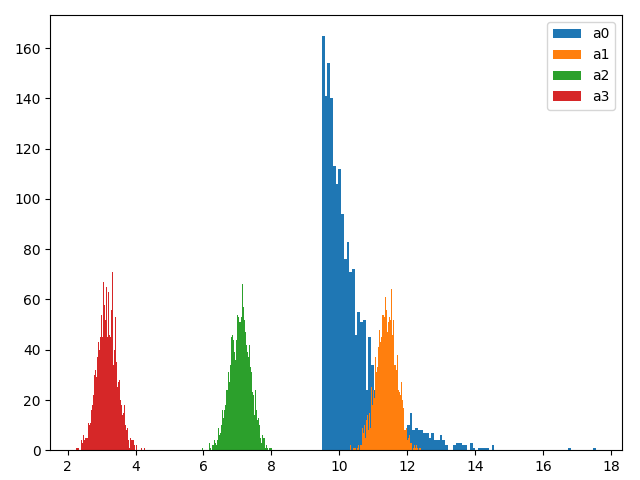
\includegraphics[width=0.8\textwidth]{figures/1_2_1.png}
	\caption{Histograms for Scenario 2}
	\label{1_2_1}
\end{figure}
  
\textbf{Discussion}

Data from anchor $0$ ``seems'' to be \textbf{exponentially} distributed whereas
the others are look like a normal distribution.
  
  \item Maximum Likelihood for exponential distribution
  
\begin{align*}
\textnormal{Case II Exponential}: p(r_i|\mathbf{p}) = 
\begin{cases}
\lambda_i e^{-\lambda_i(r_i-d_i(\mathbf{p}))}, & r_i \geq d_i(\mathbf{p})\\
0 & \text{else}
\end{cases}
\end{align*}
and
\begin{align*}
\mathbf{\hat{p}}_{ML}=\arg\max_{\textbf{p}} p(\textbf{r}|\textbf{p}) = 
\arg\max_{\textbf{p}}\prod_{i=1}^{N_A}p(r_i|\textbf{p})
\end{align*}

We are using $\log$-Likelihood for easier derivation. This is possible since we
only want the $\max$ for the arguments and not any probability values
themselfs \autocite[9]{lecuter_notes_spsc}.

\begin{align*}
\lambda_{ML}&=\arg\max_{\lambda}L(r|\lambda)\\
L(R|\lambda)&=\sum_{i=1}^N \ln(\mathit{Exp}(r_i|\lambda))\quad\textnormal{ln
helps with }e\textnormal{ in } \mathit{Exp}\\
\frac{\partial L(r|\lambda)}{\partial\lambda} &\stackrel{!}{=} 0\\
&=\frac{\partial}{\partial\lambda}\sum_{i=1}^N \ln(\lambda_i
e^{-\lambda(r_i-d_i(\mathbf{p}))})\\
&=\frac{N}{\lambda}-\left(\sum_{i=1}^N\left(r_i-d_i(\mathbf{p})\right)\right)\\
\implies \lambda &= \frac{N}{\sum_{i=1}^N\left(r_i-d_i(\mathbf{p})\right)} 
\end{align*}


  \item Parameter Estimation

\textbf{Scenario 1}

\begin{figure}[H]
  \centering
  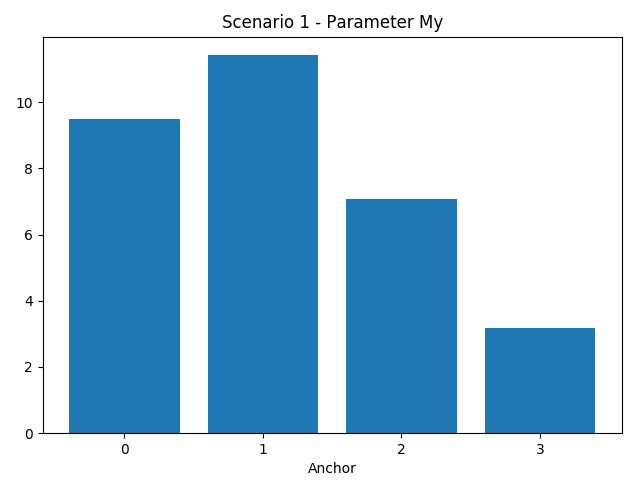
\includegraphics[width=0.6\textwidth]{figures/1_2_3_1_my.png}
	\caption{Parameter Estimation Scenario 1 - Parameter $\mu$}
	\label{1_2_3_1_my}
\end{figure}

\begin{figure}[H]
  \centering
  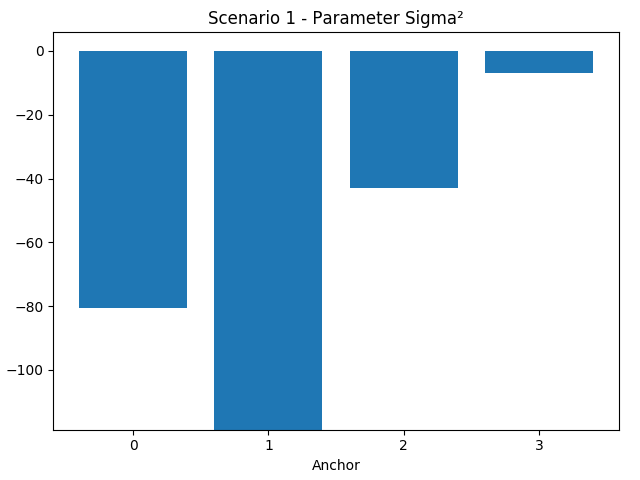
\includegraphics[width=0.6\textwidth]{figures/1_2_3_1_sigma.png}
	\caption{Parameter Estimation Scenario 1 - Parameter $\sigma^2$}
	\label{1_2_3_1_sigma}
\end{figure}

\begin{tabular}{|l|c|c|c|c|} 
 \hline
 Parameter & Anchor 1 & Anchor 2 & Anchor 3 & Anchor 4\\\hline
 $\mu$ & $9.48795736$ & $11.40808013$ & $7.08071941$ & $3.16140767$ \\\hline
 $\sigma^2$ & $-80.53337746$ & $-118.73621222$ & $-43.05586795$ & $-6.83309077$
 \\\hline
\end{tabular}

\textbf{Scenario 2}

\begin{tabular}{|l|c|c|c|c|} 
 \hline
 Parameter & Anchor 1 & Anchor 2 & Anchor 3 & Anchor 4\\\hline
 $\mu$ & $-$ & $11.39544817$ & $7.0798979$ & $3.16310352$ \\\hline
 $\sigma^2$ & $-$ & $-118.46079088$ & $-43.04505635$ & $-6.84212036$
 \\\hline
 $\lambda$ & $-3.82138765e^{-16}$ & $-$ & $-$
 & $-$ \\\hline
\end{tabular}

\textbf{Scenario 3}

\begin{figure}[H]
  \centering
  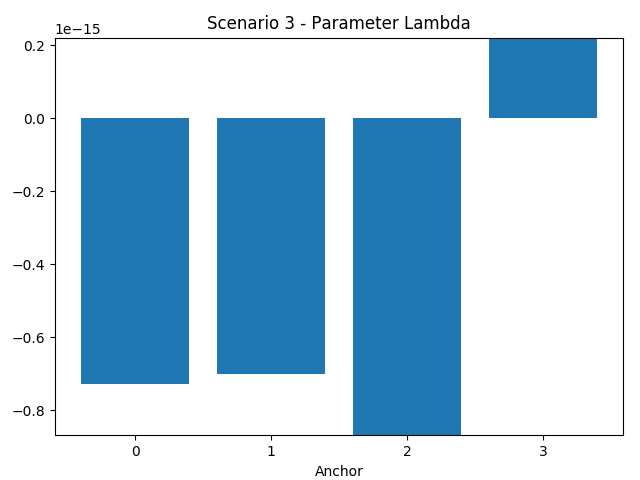
\includegraphics[width=0.6\textwidth]{figures/1_2_3_3_lambda.png}
	\caption{Parameter Estimation Scenario 3 - Parameter $\lambda$}
	\label{1_2_3_3_lambda}
\end{figure}

\begin{tabular}{|l|c|c|c|c|} 
 \hline
 Parameter & Anchor 1 & Anchor 2 & Anchor 3 & Anchor 4\\\hline
 $\lambda$ & $-7.27418126e^{-16}$ & $-7.00772773e^{-16}$ & $-8.68638494e^{-16}$
 & $2.21156427e^{-16}$ \\\hline
\end{tabular}

\end{enumerate}

\subsection{Least-Squares Estimation of the Position}

\begin{enumerate}[1.]
  \item $\mathbf{\hat{p}}_{ML} \stackrel{?}{=} \mathbf{\hat{p}}_{LS}$

\begin{align*}
\arg\max_{\textbf{p}}\prod_{i=1}^{N_A}p(r_i|\textbf{p}) &\stackrel{?}{=}
\arg\min_{\textbf{p}}\sum_{i=1}^{N_A}(r_i-d_i(\textbf{p}))^2
\end{align*}

Again using $\log$-Likelihood will help. Product will become
sum\autocite[9]{lecuter_notes_spsc} ($ln[\prod(x)] \rightarrow \sum[ln(x)]$).

	\item code is still bugy.
	

\end{enumerate}

\subsection{Numerical Maximum-Likelihood Estimation of the Position}

???

\newpage
\printbibliography

\end{document}